\section{Sphinx}

As illustrated in Figure \ref{fig:sphinx_structure}, the Sphinx packet consists of a header and an encrypted payload. 
The header contains a cryptographic element, encrypted routing information, and an integrity tag.
The encrypted routing information is encapsulated with an integrity check as shown in Figure \ref{fig:sphinx_header}.

\begin{figure}[h]
    \centering
    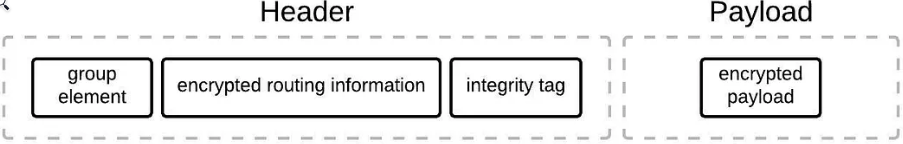
\includegraphics[width=0.9\linewidth]{Images/sphinx_structure.png}
    \caption{Structure of sphinx packet. \href{https://blog.nymtech.net/sphinx-tl-dr-the-data-packet-that-can-anonymize-bitcoin-and-the-internet-18d152c6e4dc}{[source]}}
    \label{fig:sphinx_structure}
\end{figure}

\begin{figure}[h]
    \centering
    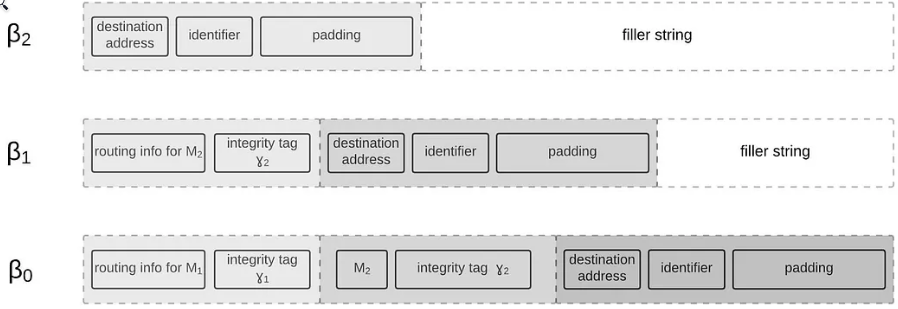
\includegraphics[width=\linewidth]{Images/sphinx_header.png}
    \caption{Sphinx encrypted routing information encapsulation. \href{https://blog.nymtech.net/sphinx-tl-dr-the-data-packet-that-can-anonymize-bitcoin-and-the-internet-18d152c6e4dc}{[source]}}
    \label{fig:sphinx_header}
\end{figure}

To encrypt the routing information, the user first chooses a random secret value $x$ and compute $g^x$ as the cryptographic element of the header.
Since each mixnode $i$ has a private key $x_i$ and a public key $y_i = g^{x_i}$, the user can create a shared secret $s_i$ with mixnode $i$ as followed: $s_i = y_i^x$. 
Then the mixnode $i$ receiving the packet will get $g^x$ allowing him to compute the shared secret as followed: $s_i = (g^x)^{x_i}$.

The encrypted routing information is computed, as illustrated in Figure \ref{fig:header_cipher}, by processing the path in reverse order. This involves XORing the current routing information ($\beta_{i-1}$) with a value derived from the shared secret $s_i$. Then prepending this new encrypted routing information ($\beta_i$) with an integrity tag ($\gamma_i$) and the previous mixnode address (remember we build it in reverse order).

\begin{figure}[H]
    \centering
    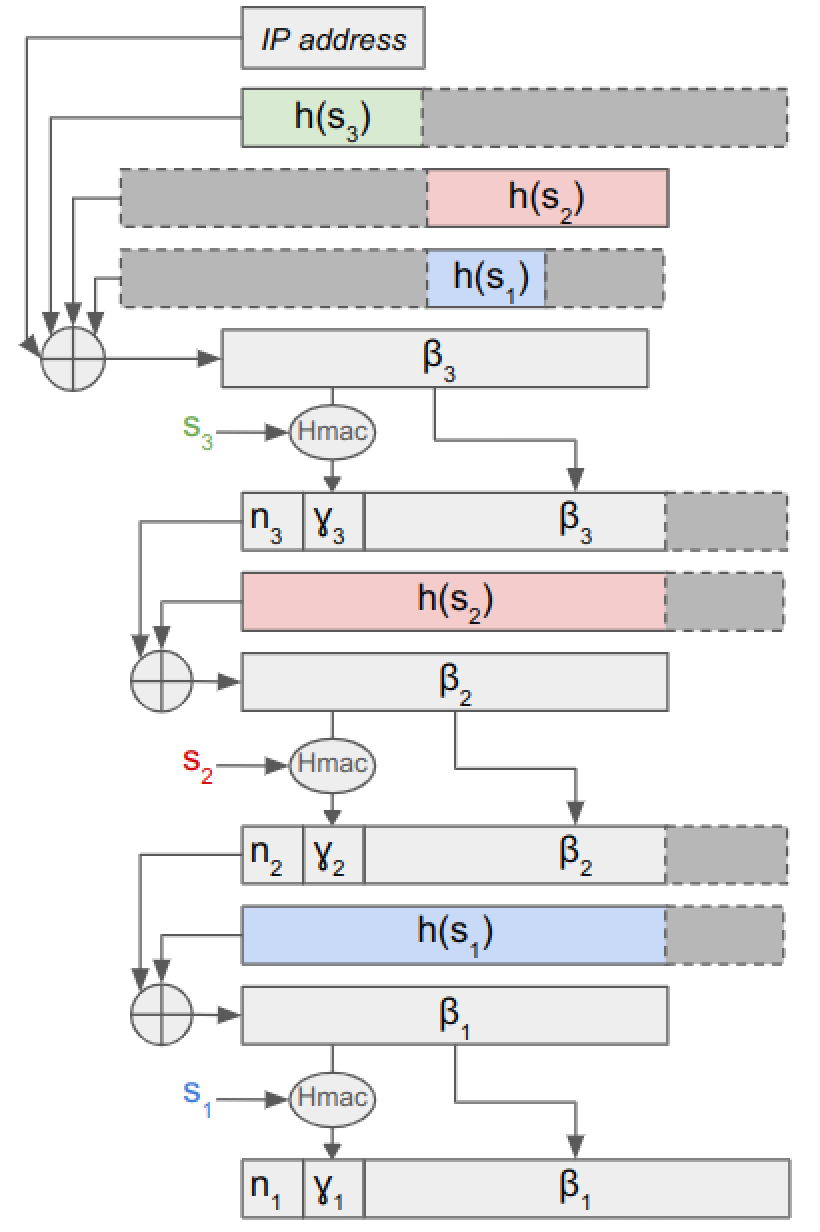
\includegraphics[width=0.5\linewidth]{Images/header_cipher.png}
    \caption{Construction of the Sphinx header (modified from \cite{sphinx})}
    \label{fig:header_cipher}
\end{figure}

We repeat the same process at each XOR step (i.e., additional nodes can easily be added to the path by following this pattern). However, the first XOR differs as it requires combining parts of all shared secrets. This deviation is a deliberate design choice to ensure fixed-size headers, enabling fixed-size packets which is a crucial property in mixnets for maintaining anonymity.



